\section{Random Forests}
\begin{multicols}{2}

A widely used and effective method in machine learning involves creating learning models known as \emph{ensembles}. An ensemble takes multiple individual learning models and combines them to produce an aggregate model that is more powerful than any of its individual learning models alone. 

Why are ensembles effective? Well, one reason is that if we have different learning models, although each of them might perform well individually, they'll tend to make different kinds of mistakes on the data set. And typically, this happens because each individual model might overfit to a different part of the data. By combining different individual models into an ensemble, we can average out their individual mistakes to reduce the risk of overfitting while maintaining strong prediction performance. 

Random forests are an example of the ensemble idea applied to decision trees. Random forests are widely used in practice and achieve very good results on a wide variety of problems. They can be used as classifiers via the sklearn \texttt{RandomForestClassifier} class or for regression using the \texttt{RandomForestRegressor} class both in the \texttt{sklearn.ensemble} module. 

As we saw earlier, one disadvantage of using a \emph{single} decision tree was that decision trees tend to be prone to overfitting the training data. 

As its name would suggest, a random forest creates lots of individual decision trees on a training set, often on the order of tens or hundreds of trees. The idea is that each of the individual trees in a random forest should do reasonably well at predicting the target values in the training set but should also be constructed to be different in some way from the other trees in the forest. 

Again, as the name would suggest this difference is accomplished by introducing random variation into the process of building each decision tree. 

\begin{center}
	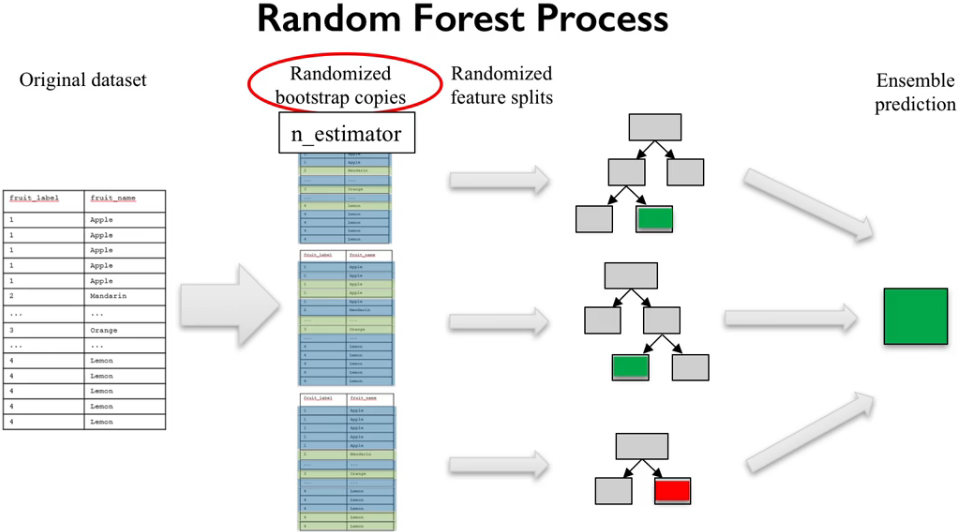
\includegraphics[width=\linewidth]{img/Random-Forest-Process.png} 
\end{center}


This random variation during tree building happens in two ways. First, the data used to build each tree is selected randomly and second, the features chosen in each split tests are also randomly selected. 

\subsection{Random Forests Model Creation}

To create a random forest model you first decide on how many trees to build. This is set using the \texttt{n_estimated} parameter for both RandomForestClassifier and RandomForestRegressor. Each tree were built from a different random sample of the data called the bootstrap sample. Bootstrap samples are commonly used in statistics and machine learning. If your training set has N instances or samples in total, a bootstrap sample of size N is created by just repeatedly picking one of the N dataset rows at random with replacement, that is, allowing for the possibility of picking the same row again at each selection. 

\begin{center}
	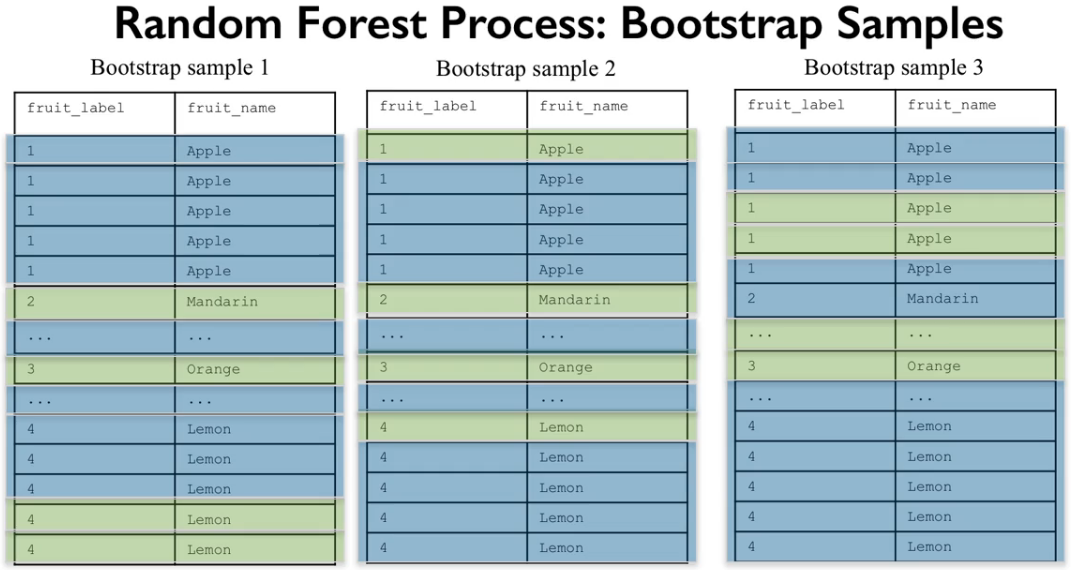
\includegraphics[width=\linewidth]{img/Bootstrap-Samples.png} 
\end{center}

You repeat this random selection process N times. The resulting bootstrap sample has N rows just like the original training set but with possibly some rows from the original dataset missing and others occurring multiple times just due to the nature of the random selection with replacement. 

When building a decision tree for a random forest, the process is almost the same as for a standard decision tree but with one important \emph{difference}. When picking the best split for a node, instead of finding the best split across all possible features, a \emph{random subset of features} is chosen and the best split is found within that smaller subset of features. The number of features in the subset that are randomly considered at each stage is controlled by the \texttt{max_features} parameter. 

This randomness in selecting the bootstrap sample to train an individual tree in a forest ensemble, combined with the fact that splitting a node in the tree is restricted to random subsets of the features of the split, virtually guarantees that all of the decision trees and the random forest will be different. 

The random forest model is quite sensitive to the \texttt{max_features} parameter. If \texttt{max_features = 1}, the random forest is limited to performing a split on the single feature that was selected randomly instead of being able to take the best split over several variables. This means the trees in the forest will likely be very different from each other and possibly with many levels in order to produce a good fit to the data. 

On the other hand if \texttt{max_features} is high, close to the total number of features that each instance has, the trees in the forest will tend to be similar and probably will require fewer levels to fit the data using the most informative features. 

\subsection{Prediction}

Once a random forest model is trained, it predicts the target value for new instances by first making a prediction for every tree in the random forest. 

\begin{center}
	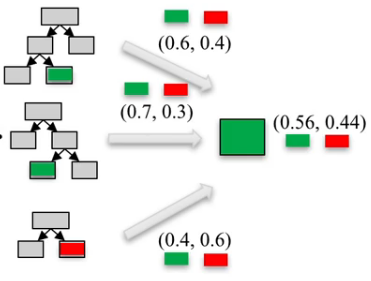
\includegraphics[width=\linewidth]{img/Random-Forest-Prediction.png} 
\end{center}

For \emph{regression} tasks the overall prediction is then typically the \textbf{mean} of the individual tree predictions. For \emph{classification} the overall prediction is based on a \textbf{weighted vote}. Each tree gives a probability for each possible target class label then the probabilities for each class are averaged across all the trees and the class with the highest probability is the final predicted class. 

\begin{center}
	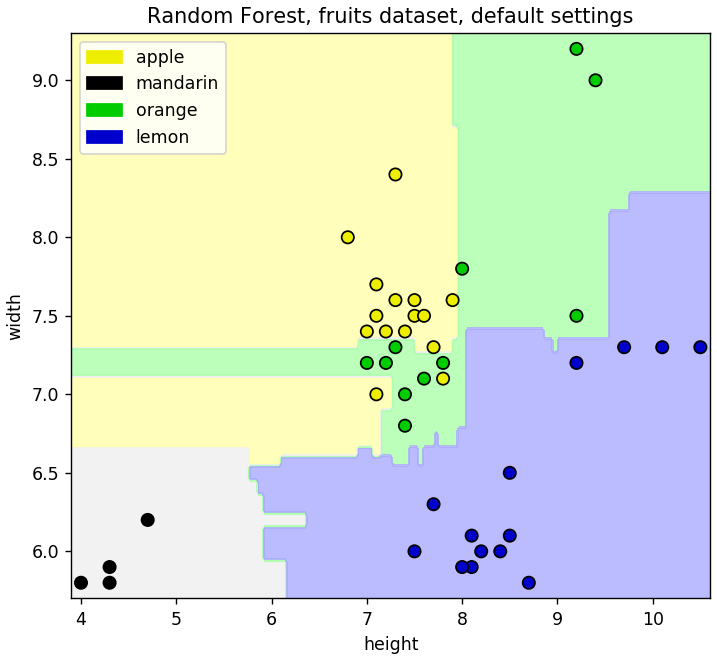
\includegraphics[width=\linewidth]{img/Random-Forest-Fruit-dataset.png} 
\end{center}

Here's an example of learning a random forest of the example fruit dataset using two features, height and width. Here we're showing the training data plotted in terms of two feature values with height on the x axis and width on the y axis. 

As usual, there are four categories of fruit to be predicted. Because the number of features is restricted to just two in this very simple example, the randomness in creating the tree ensemble is coming mostly from the bootstrap sampling of the training data. You can see that the decision boundaries overall have the \emph{box like shape} that we associate with decision trees but with some additional detail variation to accommodate specific local changes in the training data. 

Overall, you can get an impression of the increased complexity of this random forest model in capturing both the global and local patterns in the training data compared to the single decision tree model we saw earlier. 

\subsection{Implementation}

\subsubsection*{Fruit dataset}

Let's take a look at the notebook code that created and visualized this random forest on the fruit dataset.
{\scriptsize
\begin{verbatim}
from sklearn.ensemble import RandomForestClassifier
...
clf = RandomForestClassifier().fit(X, y)
clf = RandomForestClassifier(n_estimators = 10,
      random_state=0).fit(X_train, y_train)
...
Random Forest, Fruit dataset, default settings
Accuracy of RF classifier on training set: 1.00
Accuracy of RF classifier on test set: 0.80
\end{verbatim}
}

To use the \texttt{RandomForestClassifier} we import the random forest classifier class from the \texttt{sklearn.ensemble} library. 

For each pair of features we call the fit method on that subset of the training data X using the labels y. We then use the utility function plot class regions for classifier to visualize the training data and the random forest decision boundaries. 

Let's apply random forest to a larger dataset with more features. 

\subsubsection*{Breast Cancer dataset}

For comparison with other supervised learning methods, we use the breast cancer dataset. We create a new random forest classifier and since there are about 30 features, we'll set \texttt{max_features~=~8} to give a diverse set of trees that also fit the data reasonably well. 

{\scriptsize
\begin{verbatim}
Breast cancer dataset
Accuracy of RF classifier on training set: 1.00
Accuracy of RF classifier on test set: 0.99
\end{verbatim}
}

We can see that random forest with no feature scaling or extensive parameter tuning achieve very good test set performance on this dataset, in fact, it's as good or better than all the other supervised methods we've seen so far including current life support vector machines and neural networks that require more careful tuning. 

\textbf{Notice} that we did not have to perform scaling or other pre-processing as we did with a number of other supervised learning methods. This is one \emph{advantage} of using random forests. 

\subsection{Pros and Cons}

On the \textbf{positive} side of Random Forests:
\begin{itemize}
\item widely used, excellent prediction performance on many problems;
\item doesn't require careful normalization of features or extensive paramener tuning;
\item like decision trees, handles a mixture of feature types;
\item easily parallelized across multiple CPUs.
\end{itemize}

Even though building many different trees requires a corresponding increase in computation, building random forests is easily parallelized across multiple CPU's. 


On the \textbf{negative} side:
\begin{itemize}
\item the resulting modela are often difficult for humans to interpret~--- difficult to see the predictive structure of the features or to know why a particular prediction was made;
\item not a good choice for tasks that have very high dimensional sparse features like text classification.
\end{itemize}

\subsection{Key Parameters}

Here are some of the key parameters that you'll need for using random forests. 

\texttt{N_estimators} sets the number of trees to use. The default value for \texttt{n_estimators}~= 10 and increasing this number for larger data sets is almost certainly a good idea since ensembles that can average over more trees will reduce overfitting. 

Just bear in mind that increasing the number of trees in the model will also increase the computational cost of training. You'll use more time and more memory. So in practice you'll want to choose the parameters that make best use of the resources available on your system. 

The \texttt{max_features} parameter has a strong effect on performance. It has a large influence on how diverse the random trees in the forest are. Typically, the default setting of \texttt{max_features}, which for classification is the square root of the total number of features and for regression is the log base two of the total number of features, works quite well in practice although explicitly adjusting \texttt{max_features} may give you some additional performance gain with smaller values of max features tending to reduce overfitting. 

The \texttt{max_depth} parameter controls the depth of each tree in the ensemble. The default setting for this is none, in other words, the nodes in a tree will continue to be split until all leaves contain the same class or have fewer samples than the minimum sample split parameter value, which is two by default. 

The \texttt{n_jobs} parameter~--- how many cores to use in parallel to train the model. Generally, you can expect something close to a linear speed up. So, for example, if you have four cores, the training will be four times as fast as if you just used one. If you set end jobs to negative one it will use all the cores on your system and setting end jobs to a number that's more than the number of cores on your system won't have any additional effect. 

\end{multicols}